\documentclass[10pt,a4paper]{article}

\usepackage[landscape,margin=0.55in]{geometry}
\usepackage[T1]{fontenc}
\usepackage{lmodern}
\usepackage{microtype}
\usepackage[dvipsnames]{xcolor}
\usepackage{tikz}
\usetikzlibrary{arrows.meta,positioning,calc,shapes.geometric}
\usepackage[most]{tcolorbox}
\usepackage{tabularx,array,booktabs,multicol}
\usepackage{enumitem}
\usepackage{amssymb}
\usepackage{hyperref}
\hypersetup{colorlinks=false,pdfborder={0 0 0}}
\pagestyle{empty}
\setlength{\parindent}{0pt}
\setlength{\parskip}{3pt}
\renewcommand{\arraystretch}{1.25}

% ------------------ Colors ------------------
\definecolor{Ink}{HTML}{111111}
\definecolor{SoftInk}{HTML}{333333}
\definecolor{Rule}{HTML}{222222}
\definecolor{LightPanel}{HTML}{F5F5F2}
\definecolor{MidPanel}{HTML}{E9E9E4}
\definecolor{DarkPanel}{HTML}{202020}
\definecolor{Accent}{HTML}{2F5D50}
\definecolor{AccentLight}{HTML}{EAF3F0}
\definecolor{Warm}{HTML}{F8F3E8}
\definecolor{LineGrey}{HTML}{C9C9C3}
\definecolor{GreenSoft}{HTML}{E8F5E9}
\definecolor{OrangeSoft}{HTML}{FFF3E0}
\definecolor{BlueSoft}{HTML}{EAF2FF}
\definecolor{RedSoft}{HTML}{FDECEC}

% ------------------ General styles ------------------
\tcbset{
  basebox/.style={
    enhanced,
    colback=white,
    colframe=Rule,
    boxrule=0.7pt,
    arc=2mm,
    left=3mm,right=3mm,top=2.5mm,bottom=2.5mm,
    fonttitle=\bfseries\large,
    coltitle=white,
    colbacktitle=Ink,
    attach boxed title to top left={xshift=3mm,yshift*=-2mm},
    boxed title style={sharp corners,boxrule=0pt,arc=1mm,left=2mm,right=2mm,top=1mm,bottom=1mm}
  },
  usebox/.style={basebox,colback=LightPanel},
  blankbox/.style={basebox,colback=white},
  smallbox/.style={basebox,fonttitle=\bfseries\normalsize},
}

\newcommand{\CheckLine}{\raisebox{0.2ex}{\Large$\square$}\hspace{1mm}}
\newcommand{\FillLine}{\makebox[0.82\linewidth]{\hrulefill}}
\newcommand{\minihead}[1]{\vspace{1mm}\textbf{#1}\par}
\newcommand{\pagetitle}[2]{%
  {\fontsize{26}{29}\selectfont\bfseries #1}\par
  {\large\color{SoftInk}#2}\par\vspace{3mm}\hrule\vspace{4mm}
}
\newcommand{\boardfooter}{\vfill\begin{center}\small Keep this page visible. Use pencil. Review once at the end of the day.\end{center}}

% ------------------ TikZ templates ------------------
\newcommand{\PomodoroCycle}{%
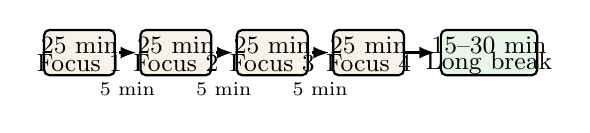
\begin{tikzpicture}[scale=0.72, every node/.style={font=\small}]
  \foreach \x/\lab in {0/1,1.7/2,3.4/3,5.1/4}{
    \draw[thick,rounded corners=2pt,fill=Warm] (\x,0) rectangle +(1.25,0.8);
    \node at (\x+0.625,0.53) {25 min};
    \node at (\x+0.625,0.22) {Focus \lab};
  }
  \foreach \x in {1.25,2.95,4.65}{\draw[-{Latex[length=2mm]},thick] (\x+0.08,0.4)--+(0.3,0);\node[below,font=\scriptsize] at (\x+0.22,0.05) {5 min};}
  \draw[-{Latex[length=2mm]},thick] (6.35,0.4)--+(0.55,0);
  \draw[thick,rounded corners=2pt,fill=GreenSoft] (7.0,0) rectangle +(1.7,0.8);
  \node at (7.85,0.53) {15--30 min};
  \node at (7.85,0.22) {Long break};
\end{tikzpicture}}

\newcommand{\EisenhowerMatrix}{%
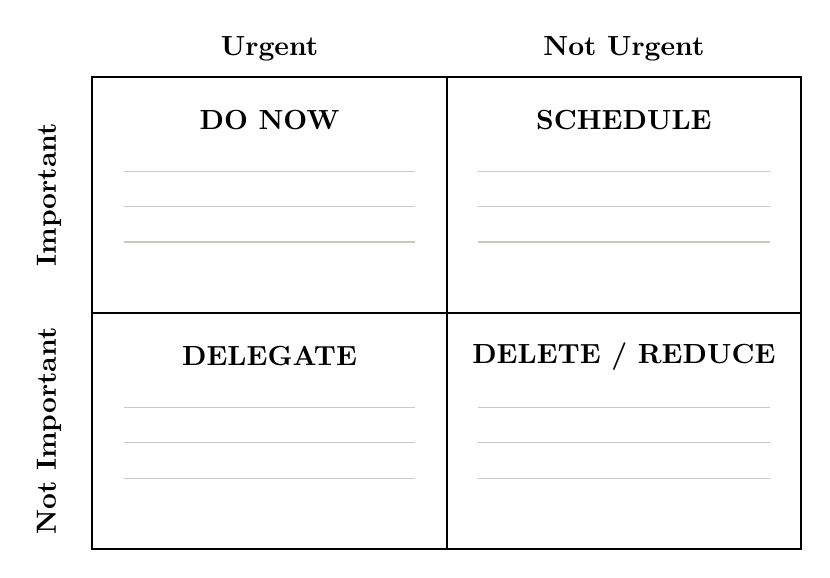
\begin{tikzpicture}[x=1cm,y=1cm, every node/.style={font=\small}]
  \draw[thick] (0,0) rectangle (9,6);
  \draw[thick] (4.5,0)--(4.5,6);
  \draw[thick] (0,3)--(9,3);
  \node[font=\bfseries] at (2.25,6.35) {Urgent};
  \node[font=\bfseries] at (6.75,6.35) {Not Urgent};
  \node[rotate=90,font=\bfseries] at (-0.55,4.5) {Important};
  \node[rotate=90,font=\bfseries] at (-0.55,1.5) {Not Important};
  \node[align=center,font=\bfseries] at (2.25,5.45) {DO NOW};
  \node[align=center,font=\bfseries] at (6.75,5.45) {SCHEDULE};
  \node[align=center,font=\bfseries] at (2.25,2.45) {DELEGATE};
  \node[align=center,font=\bfseries] at (6.75,2.45) {DELETE / REDUCE};
  \foreach \y in {4.8,4.35,3.9,1.8,1.35,0.9}{\draw[LineGrey] (0.4,\y)--(4.1,\y);\draw[LineGrey] (4.9,\y)--(8.6,\y);}
\end{tikzpicture}}

\newcommand{\ThreeThreeThree}{%
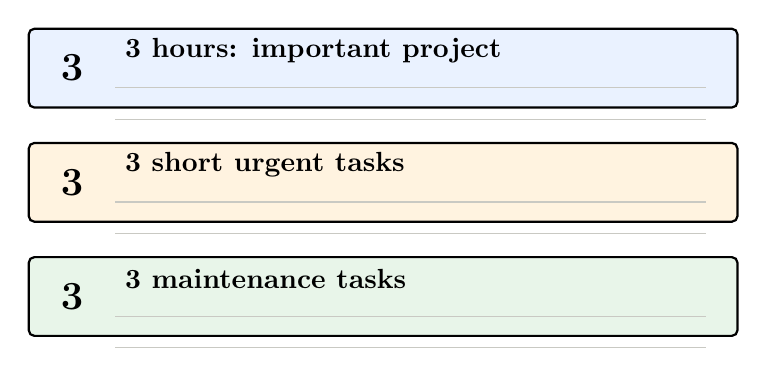
\begin{tikzpicture}[x=1cm,y=1cm, every node/.style={font=\small}]
  \foreach \i/\title/\fill in {0/3 hours: important project/BlueSoft,1/3 short urgent tasks/OrangeSoft,2/3 maintenance tasks/GreenSoft}{
    \draw[thick,rounded corners=2pt,fill=\fill] (0,-\i*1.45) rectangle (9,1.0-\i*1.45);
    \node[font=\bfseries\Large] at (0.55,0.5-\i*1.45) {3};
    \node[anchor=west,font=\bfseries] at (1.1,0.72-\i*1.45) {\title};
    \draw[LineGrey] (1.1,0.25-\i*1.45)--(8.6,0.25-\i*1.45);
    \draw[LineGrey] (1.1,-0.15-\i*1.45)--(8.6,-0.15-\i*1.45);
  }
\end{tikzpicture}}

\newcommand{\PARAFigure}{%
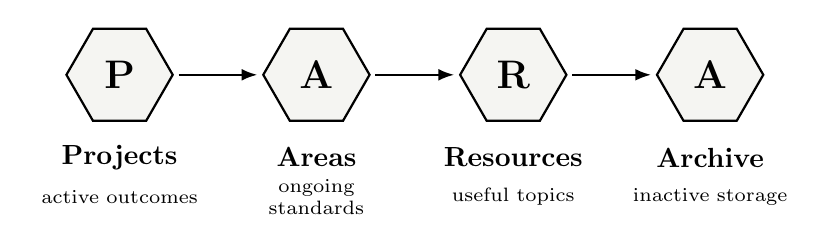
\begin{tikzpicture}[x=1cm,y=1cm, every node/.style={font=\small}]
  \foreach \x/\letter/\name/\desc in {0/P/Projects/active outcomes,2.5/A/Areas/ongoing standards,5/R/Resources/useful topics,7.5/A/Archive/inactive storage}{
    \node[draw,regular polygon,regular polygon sides=6,minimum size=1.35cm,thick,fill=LightPanel,font=\bfseries\Large] (n\letter\x) at (\x,0) {\letter};
    \node[font=\bfseries,align=center] at (\x,-1.05) {\name};
    \node[align=center,text width=2.1cm,font=\scriptsize] at (\x,-1.55) {\desc};
  }
  \draw[-{Latex[length=2mm]},thick] (0.75,0)--(1.75,0);
  \draw[-{Latex[length=2mm]},thick] (3.25,0)--(4.25,0);
  \draw[-{Latex[length=2mm]},thick] (5.75,0)--(6.75,0);
\end{tikzpicture}}

\newcommand{\FlowVenn}{%
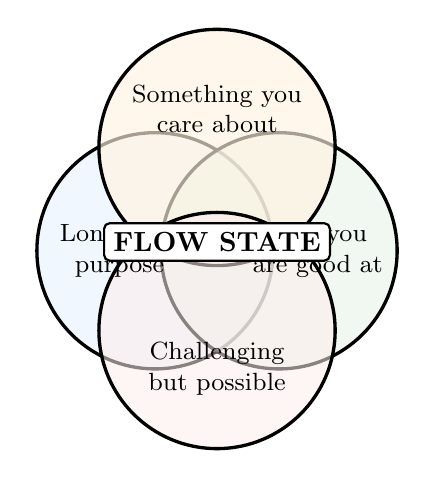
\begin{tikzpicture}[scale=0.75, every node/.style={font=\small}]
  \draw[very thick,fill=BlueSoft,fill opacity=.65] (0,0) circle (2.0);
  \draw[very thick,fill=GreenSoft,fill opacity=.65] (2.1,0) circle (2.0);
  \draw[very thick,fill=OrangeSoft,fill opacity=.65] (1.05,1.75) circle (2.0);
  \draw[very thick,fill=RedSoft,fill opacity=.55] (1.05,-1.35) circle (2.0);
  \node[align=center,text width=2.1cm] at (-0.6,0) {Long-term\ purpose};
  \node[align=center,text width=2.1cm] at (2.75,0) {Skill you\ are good at};
  \node[align=center,text width=2.2cm] at (1.05,2.4) {Something\ you care about};
  \node[align=center,text width=2.2cm] at (1.05,-2.0) {Challenging\ but possible};
  \node[draw,thick,rounded corners=2pt,fill=white,align=center,font=\bfseries] at (1.05,0.15) {FLOW\ STATE};
\end{tikzpicture}}

\newcommand{\ParkinsonCurve}{%
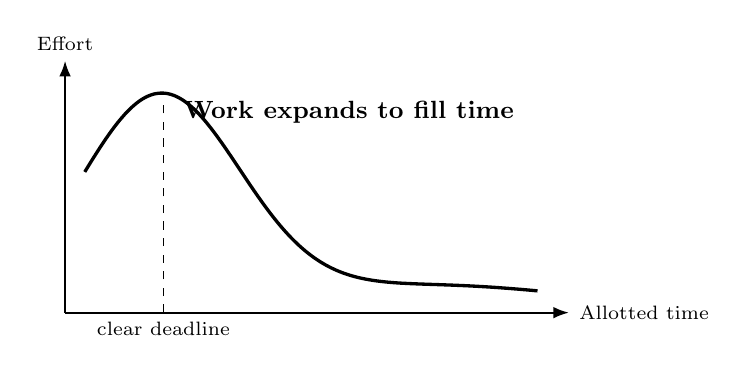
\begin{tikzpicture}[x=1cm,y=1cm, every node/.style={font=\scriptsize}]
  \draw[-{Latex[length=2mm]},thick] (0,0)--(6.4,0) node[right]{Allotted time};
  \draw[-{Latex[length=2mm]},thick] (0,0)--(0,3.2) node[above]{Effort};
  \draw[very thick,domain=0.25:6,smooth,samples=80] plot (\x,{2.7*exp(-0.48*(\x-1.2)*(\x-1.2))+0.35*exp(-0.12*(\x-4.6)*(\x-4.6))});
  \draw[dashed] (1.25,0)--(1.25,2.7);
  \node[below] at (1.25,0) {clear deadline};
  \node[align=center,font=\small\bfseries] at (3.6,2.55) {Work expands\ to fill time};
\end{tikzpicture}}

% ------------------ Document ------------------
\begin{document}

% ============================================================

\pagetitle{Productivity Notice Board}{A practical wall-sheet: choose one method, write today's items, act, and review.}

\begin{tcolorbox}[usebox,title={How to use this board}]
\begin{multicols}{3}
\textbf{1. Start with clarity.} Write the single most important outcome of the day. Do not begin with random messages or social media.\par
\textbf{2. Sort the work.} Use the Eisenhower Matrix to separate important work from noise.\par
\textbf{3. Work in blocks.} Use Pomodoro for focus, 3/3/3 for a balanced day, and Time Blocking for a visible timetable.\par
\textbf{4. Keep a streak.} Mark one daily habit or project action on the calendar. Never miss two days in a row.\par
\textbf{5. Capture ideas.} Put notes into Projects, Areas, Resources, or Archive so they do not remain scattered.\par
\textbf{6. Review briefly.} At night, tick completed work, move unfinished work, and prepare tomorrow's first task.
\end{multicols}
\end{tcolorbox}

\vspace{2mm}
\begin{tcolorbox}[blankbox,title={Six methods at a glance}]
\begin{tabularx}{\linewidth}{>{\bfseries}p{0.18\linewidth}X p{0.25\linewidth}}
\toprule
Method & Best use & Daily action \\
\midrule
Pomodoro & Starting a task when the mind is scattered. & 25 minutes focused work + 5 minutes break. Repeat four times. \\
3/3/3 Method & Creating a balanced day without overplanning. & 3 hours deep project, 3 urgent tasks, 3 maintenance tasks. \\
Eisenhower Matrix & Deciding what deserves attention first. & Do, schedule, delegate, or eliminate. \\
Eat the Frog & Ending procrastination on the hardest task. & Do the most difficult meaningful task first. \\
Seinfeld Strategy & Building consistency in writing, study, exercise, or research. & Mark a visible calendar every day you complete the habit. \\
Time Blocking & Protecting focus from interruptions. & Assign a fixed time slot to each major activity. \\
\bottomrule
\end{tabularx}
\end{tcolorbox}

\vspace{2mm}
\begin{tcolorbox}[blankbox,title={Daily decision rule}]
\Large
If a task is \textbf{important and urgent}, do it now. If it is \textbf{important but not urgent}, schedule it. If it is \textbf{urgent but not important}, delegate or shorten it. If it is neither, remove it.
\end{tcolorbox}
\begin{center}\small Keep this page visible. Use pencil. Review once at the end of the day.\end{center}

% ============================================================

\newpage


\pagetitle{Daily Execution Template}{Print this page daily or pin one laminated copy and write with marker.}
{\footnotesize
\begin{minipage}[t]{0.32\linewidth}
\begin{tcolorbox}[usebox,title={1. Main outcome and frog task}]
\textbf{Main outcome:}\par\vspace{2mm}\rule{0.96\linewidth}{0.35pt}\par\vspace{3mm}
\textbf{Why it matters:}\par\vspace{2mm}\rule{0.96\linewidth}{0.35pt}\par\vspace{3mm}
\textbf{Hardest meaningful task first:}\par\vspace{2mm}\rule{0.96\linewidth}{0.35pt}\par\vspace{2mm}
Start time: \rule{25mm}{0.35pt}\hfill Finish: \rule{25mm}{0.35pt}
\end{tcolorbox}

\begin{tcolorbox}[usebox,title={2. Pomodoro work log}]
\centering\PomodoroCycle\par\vspace{1mm}
\begin{tabularx}{\linewidth}{c X c}
\textbf{Round} & \textbf{Task} & \textbf{Done}\\\hline
1 & & $\square$\\
2 & & $\square$\\
3 & & $\square$\\
4 & & $\square$\\
\end{tabularx}
\end{tcolorbox}
\end{minipage}\hfill
\begin{minipage}[t]{0.32\linewidth}
\begin{tcolorbox}[usebox,title={3. 3/3/3 balanced day}]
\textbf{3 hours - important project}\par\rule{0.96\linewidth}{0.35pt}\par\vspace{1.5mm}
\textbf{3 shorter urgent tasks}\par
$\square$ \rule{0.82\linewidth}{0.35pt}\par
$\square$ \rule{0.82\linewidth}{0.35pt}\par
$\square$ \rule{0.82\linewidth}{0.35pt}\par\vspace{1.5mm}
\textbf{3 maintenance tasks}\par
$\square$ \rule{0.82\linewidth}{0.35pt}\par
$\square$ \rule{0.82\linewidth}{0.35pt}\par
$\square$ \rule{0.82\linewidth}{0.35pt}
\end{tcolorbox}

\begin{tcolorbox}[usebox,title={4. Time blocking}]
\begin{tabularx}{\linewidth}{p{0.24\linewidth}X c}
\textbf{Time} & \textbf{Block} & \textbf{Done}\\\hline
6--8 & & $\square$\\
8--10 & & $\square$\\
10--12 & & $\square$\\
12--2 & & $\square$\\
2--4 & & $\square$\\
4--6 & & $\square$\\
6--9 & & $\square$\\
\end{tabularx}
\end{tcolorbox}
\end{minipage}\hfill
\begin{minipage}[t]{0.32\linewidth}
\begin{tcolorbox}[usebox,title={5. Distraction control}]
$\square$ Phone away or on silent\par
$\square$ Notifications off\par
$\square$ Desk cleared\par
$\square$ Water and materials ready\par
$\square$ One tab / one notebook only
\end{tcolorbox}

\begin{tcolorbox}[usebox,title={6. End-of-day review}]
\textbf{Completed:}\par\rule{0.96\linewidth}{0.35pt}\par\vspace{2mm}
\textbf{Postponed:}\par\rule{0.96\linewidth}{0.35pt}\par\vspace{2mm}
\textbf{Tomorrow's first task:}\par\rule{0.96\linewidth}{0.35pt}\par\vspace{2mm}
\textbf{Improve tomorrow:}\par\rule{0.96\linewidth}{0.35pt}
\end{tcolorbox}

\begin{tcolorbox}[usebox,title={7. Daily score}]
\begin{tabularx}{\linewidth}{X c}
Main outcome attempted & $\square$\\
Frog task started & $\square$\\
Two focus blocks completed & $\square$\\
Distractions reduced & $\square$\\
Tomorrow planned & $\square$\\
\end{tabularx}
\end{tcolorbox}
\end{minipage}
}
% ============================================================

\newpage

\pagetitle{Eisenhower Matrix Template}{Use this before starting the day, before meetings, or when too many tasks feel equally important.}

\begin{minipage}[t]{0.46\linewidth}
\begin{tcolorbox}[blankbox,title={Blank matrix for today's tasks}]
\centering\EisenhowerMatrix
\end{tcolorbox}
\end{minipage}\hfill
\begin{minipage}[t]{0.50\linewidth}
\begin{tcolorbox}[usebox,title={How to fill it}]
\begin{enumerate}[leftmargin=5mm,itemsep=2mm]
\item Write every pending task quickly without judging it.
\item Ask: \textbf{Will this matter after one week or one month?} If yes, it is probably important.
\item Ask: \textbf{Will there be a real cost if I delay it today?} If yes, it is urgent.
\item Put each task into one box. Do not put everything in \emph{Do Now}.
\item Start only with the top-left box, then schedule the top-right box.
\end{enumerate}
\end{tcolorbox}

\begin{tcolorbox}[usebox,title={Examples}]
\begin{tabularx}{\linewidth}{>{\bfseries}p{0.28\linewidth}X}
Do now & Deadline today, important official reply, urgent health or family matter.\\
Schedule & Research writing, lecture preparation, exercise, financial planning, skill learning.\\
Delegate / ask help & Routine paperwork, formatting, repeated admin work, task someone else can handle.\\
Delete / reduce & Random scrolling, unnecessary perfection, low-value meetings, repeated checking.\\
\end{tabularx}
\end{tcolorbox}

\begin{tcolorbox}[usebox,title={Notice-board reminder}]
A task is not important just because it is loud. A task is important when it protects health, family, career, learning, responsibility, or long-term peace.
\end{tcolorbox}
\end{minipage}

% ============================================================

\newpage

\pagetitle{Focus and Work Compression}{A practical version of ``finish more in less time'' without rushing or lowering quality.}

\begin{minipage}[t]{0.48\linewidth}
\begin{tcolorbox}[usebox,title={Block out your day}]
Focus on one category of work during one dedicated block. Group similar activities together so the mind does not repeatedly switch context.\par\vspace{2mm}
\begin{tabularx}{\linewidth}{p{0.22\linewidth}X}
\textbf{Block} & \textbf{Purpose}\\\hline
Deep work & Thinking, writing, solving, preparing, designing.\\
Admin & Email, forms, bills, official replies, routine coordination.\\
People & Meetings, calls, mentoring, discussion.\\
Personal & Food, health, family, rest, commute.\\
Review & Plan tomorrow and close open loops.\\
\end{tabularx}
\end{tcolorbox}

\begin{tcolorbox}[usebox,title={Parkinson's Law: set artificial deadlines}]
\centering\ParkinsonCurve\par\vspace{2mm}
Work often expands to fill the time available. Give each task a smaller, believable deadline: \textbf{first draft in 40 minutes}, \textbf{reply batch in 20 minutes}, \textbf{outline in 15 minutes}.
\end{tcolorbox}
\end{minipage}\hfill
\begin{minipage}[t]{0.48\linewidth}
\begin{tcolorbox}[usebox,title={Find your work style}]
Choose a style for the day instead of forcing one routine every day.
\begin{tabularx}{\linewidth}{>{\bfseries}p{0.24\linewidth}X}
Planner & Writes blocks hour by hour and follows a visible schedule.\\
Prioritizer & Uses a short to-do list and finishes the most important item first.\\
Arranger & Groups similar work and keeps the day flexible.\\
Visualizer & Uses diagrams, boards, sticky notes, and checklists.\\
\end{tabularx}
\end{tcolorbox}

\begin{tcolorbox}[usebox,title={Compression checklist}]
\CheckLine I know the exact output required.\par
\CheckLine I have removed extra tabs, apps, and noise.\par
\CheckLine I have set a small deadline.\par
\CheckLine I will stop polishing after the useful version is ready.\par
\CheckLine I will review quality once, not repeatedly.
\end{tcolorbox}

\begin{tcolorbox}[usebox,title={Important note}]
No productivity method works if attention is continuously broken. Protect attention first; then choose a method.
\end{tcolorbox}
\end{minipage}

% ============================================================

\newpage

\pagetitle{Consistency and Six-Month Reset}{For long-term goals: writing, research, fitness, reading, business, exam preparation, or skill-building.}

\begin{minipage}[t]{0.48\linewidth}
\begin{tcolorbox}[usebox,title={Anti-vision to vision}]
\textbf{Anti-vision:} a clear picture of the life, habits, and outcomes you do not want. It creates urgency by showing the cost of drifting.\par\vspace{2mm}
\textbf{Vision:} the opposite direction - the meaningful life and work you are building.\par\vspace{3mm}
\begin{tabularx}{\linewidth}{X X}
\textbf{I do not want} & \textbf{Therefore I will build}\\\hline
\rule{0pt}{7mm} & \\
\rule{0pt}{7mm} & \\
\rule{0pt}{7mm} & \\
\rule{0pt}{7mm} & \\
\end{tabularx}
\end{tcolorbox}

\begin{tcolorbox}[usebox,title={Disappear for six months}]
This does not mean cutting responsibility. It means reducing low-value visibility and giving serious time to the system that supports your goal.\par\vspace{2mm}
\CheckLine Reduce social media and unnecessary comparison.\par
\CheckLine Keep one primary project visible.\par
\CheckLine Build a daily routine around fundamentals.\par
\CheckLine Avoid explaining every step to everyone.\par
\CheckLine Let visible progress speak after months.
\end{tcolorbox}
\end{minipage}\hfill
\begin{minipage}[t]{0.48\linewidth}
\begin{tcolorbox}[usebox,title={Seinfeld Strategy: don't break the chain}]
\textbf{Goal:} \FillLine\par\vspace{2mm}
\textbf{Minimum daily action:} \FillLine\par\vspace{2mm}
\begin{center}
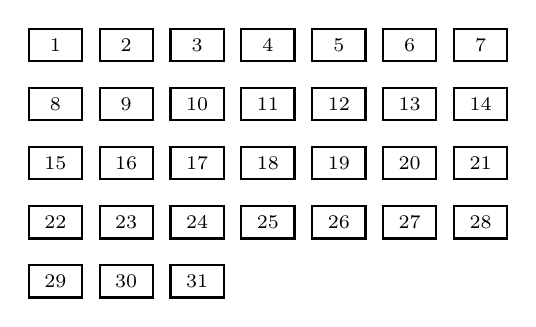
\begin{tikzpicture}[x=0.9cm,y=0.75cm, every node/.style={font=\scriptsize}]
  \foreach \d in {1,...,31}{
    \pgfmathtruncatemacro{\col}{mod(\d-1,7)}
    \pgfmathtruncatemacro{\row}{floor((\d-1)/7)}
    \draw[thick] (\col,-\row) rectangle +(0.75,-0.55);
    \node at (\col+0.375,-\row-0.275) {\d};
  }
\end{tikzpicture}
\end{center}
\textbf{Rule:} Mark the box when the minimum daily action is done. Never miss two days in a row.
\end{tcolorbox}

\begin{tcolorbox}[usebox,title={Master the fundamentals}]
Progress usually comes from repeated basic actions: reading daily, writing daily, exercising consistently, solving problems, practicing communication, tracking money, and keeping commitments. Fundamentals look boring, but they compound.
\end{tcolorbox}
\end{minipage}

% ============================================================

\newpage

\pagetitle{Organize Ideas with P.A.R.A.}{A simple template for turning scattered notes into usable knowledge.}

\begin{minipage}[t]{0.48\linewidth}
\begin{tcolorbox}[usebox,title={The P.A.R.A. flow}]
\centering\PARAFigure\par\vspace{3mm}
\begin{tabularx}{\linewidth}{>{\bfseries}p{0.22\linewidth}X}
Projects & Short-term work with an outcome and deadline. Example: prepare a lecture, finish a chapter, submit a form.\\
Areas & Ongoing responsibilities to maintain. Example: health, finances, teaching, family, department work.\\
Resources & Useful material organized by topic. Example: articles, methods, diagrams, references, templates.\\
Archive & Completed or inactive material kept for future reference.\\
\end{tabularx}
\end{tcolorbox}

\begin{tcolorbox}[usebox,title={Basic principle}]
Do not only store information. Capture it, organize it, distill it, and express it in useful work. A second brain is valuable only when it improves decisions, learning, writing, teaching, or execution.
\end{tcolorbox}
\end{minipage}\hfill
\begin{minipage}[t]{0.48\linewidth}
\begin{tcolorbox}[usebox,title={Weekly idea review template}]
\begin{tabularx}{\linewidth}{p{0.23\linewidth}X}
\textbf{Inbox notes} & \rule{0pt}{10mm}\\\hline
\textbf{Move to Project} & \rule{0pt}{10mm}\\\hline
\textbf{Move to Area} & \rule{0pt}{10mm}\\\hline
\textbf{Move to Resource} & \rule{0pt}{10mm}\\\hline
\textbf{Archive/Delete} & \rule{0pt}{10mm}\\
\end{tabularx}
\end{tcolorbox}

\begin{tcolorbox}[usebox,title={Practical tips}]
\CheckLine Keep one capture place for quick ideas.\par
\CheckLine Review once a week, not every hour.\par
\CheckLine Name folders by action, not vague emotion.\par
\CheckLine Move completed projects to Archive.\par
\CheckLine Convert useful notes into outputs: article, class note, diagram, email, checklist, or decision.
\end{tcolorbox}
\end{minipage}

% ============================================================

\newpage

\pagetitle{Flow State Template}{Use flow for meaningful work, not for distraction. Flow needs purpose, skill, challenge, and protected attention.}

\begin{minipage}[t]{0.46\linewidth}
\begin{tcolorbox}[blankbox,title={Flow state map}]
\centering\FlowVenn
\end{tcolorbox}

\begin{tcolorbox}[usebox,title={Before entering flow}]
\CheckLine Choose a task that matters.\par
\CheckLine Define the visible output.\par
\CheckLine Make the task slightly challenging, not impossible.\par
\CheckLine Remove interruptions for at least 45--90 minutes.\par
\CheckLine Keep feedback visible: word count, solved problems, pages read, draft completed.
\end{tcolorbox}
\end{minipage}\hfill
\begin{minipage}[t]{0.50\linewidth}
\begin{tcolorbox}[usebox,title={Flow worksheet}]
\begin{tabularx}{\linewidth}{>{\bfseries}p{0.29\linewidth}X}
Something I care about & \rule{0pt}{9mm}\\\hline
Long-term purpose & \rule{0pt}{9mm}\\\hline
Skill I can use & \rule{0pt}{9mm}\\\hline
Challenge level & Easy $\square$  Medium $\square$  Hard $\square$  Too hard $\square$\\\hline
First visible output & \rule{0pt}{9mm}\\\hline
Protected time block & \rule{0pt}{9mm}\\
\end{tabularx}
\end{tcolorbox}

\begin{tcolorbox}[usebox,title={Signs of a good flow block}]
\begin{tabularx}{\linewidth}{>{\bfseries}p{0.25\linewidth}X}
Clarity & You know exactly what must be produced.\\
Focus & Attention stays with one meaningful task.\\
Challenge & The task stretches ability without causing panic.\\
Feedback & You can see progress while working.\\
Fulfilment & The work connects with a larger personal or professional purpose.\\
\end{tabularx}
\end{tcolorbox}
\end{minipage}

% ============================================================

\newpage

\pagetitle{Communication and Sales Excellence}{A notice-board checklist for presenting a product, book, course, idea, or proposal.}

\begin{minipage}[t]{0.49\linewidth}
\begin{tcolorbox}[usebox,title={1. Value proposition}]
What problem does this solve, for whom, and why is it different?\par\vspace{2mm}
\CheckLine Problem: \FillLine\par\vspace{2mm}
\CheckLine Audience: \FillLine\par\vspace{2mm}
\CheckLine Unique value: \FillLine
\end{tcolorbox}

\begin{tcolorbox}[usebox,title={2. Benefits before features}]
A feature says what it has. A benefit says how it improves the user's life or work.\par\vspace{2mm}
\begin{tabularx}{\linewidth}{X X}
\textbf{Feature} & \textbf{Benefit}\\\hline
\rule{0pt}{7mm} & \\
\rule{0pt}{7mm} & \\
\rule{0pt}{7mm} & \\
\end{tabularx}
\end{tcolorbox}

\begin{tcolorbox}[usebox,title={3. Keep the message simple}]
\CheckLine One clear sentence.\par
\CheckLine No unnecessary technical detail.\par
\CheckLine No mixed promises.\par
\CheckLine The listener can repeat the idea after hearing it once.
\end{tcolorbox}
\end{minipage}\hfill
\begin{minipage}[t]{0.49\linewidth}
\begin{tcolorbox}[usebox,title={4. Tell a compelling story}]
A strong story shows the problem, struggle, turning point, and useful result.\par\vspace{2mm}
\begin{tabularx}{\linewidth}{>{\bfseries}p{0.25\linewidth}X}
Before & \\
Problem & \\
Turning point & \\
Result & \\
Proof & \\
\end{tabularx}
\end{tcolorbox}

\begin{tcolorbox}[usebox,title={5. Know the audience}]
\CheckLine What do they already believe?\par
\CheckLine What pain or need do they have?\par
\CheckLine What language do they understand?\par
\CheckLine What objection will they raise?\par
\CheckLine What next step should they take?
\end{tcolorbox}

\begin{tcolorbox}[usebox,title={6. Improve after rejection}]
Rejection is data. Note the objection, improve the message, and try again with a clearer offer, better evidence, or a more suitable audience.
\end{tcolorbox}
\end{minipage}

\end{document}
